% %!TEX program = xelatex
\documentclass[a4paper]{oblivoir}

%%% 전처리부 (preamble)
\usepackage{intothemath}
\usepackage{fancyhdr}
\usepackage{indentfirst}
\usepackage{graphicx}
\usepackage{tcolorbox}
\usepackage[left = 2cm, right = 3cm, top = 2.5cm, bottom = 2cm, a4paper]{geometry}
\usepackage{marginnote}
\usepackage{tikz}
\usepackage{tikzpagenodes}
\usepackage{lipsum}
\usepackage{color}
\usepackage{fontspec}
\usepackage{kotex}
\usepackage{hyperref}
\hypersetup{
    colorlinks=true,
    linkcolor=blue,
    filecolor=magenta,      
    urlcolor=blue,
    pdftitle={Overleaf Example},
    pdfpagemode=FullScreen,
}
\definecolor{skyblue}{RGB}{150, 210, 250}
\definecolor{header}{RGB}{60, 120, 250}
\definecolor{subheader}{rgb}{0.19, 0.55, 0.91}

\definecolor{Axiom}{rgb}{0.0, 0.25, 0.42}
\colorlet{Definition}{blue!35!skyblue}
\definecolor{Theorem}{rgb}{0.0, 0.62, 0.42}

\setmainhangulfont[Path=FONT/]{KOPUBWORLD_BATANG_PRO_LIGHT.OTF}

%%%%%%%%%%%%%%%%% 코드 세팅 %%%%%%%%%%%%%%%%%
\definecolor{dkgreen}{rgb}{0,0.6,0}
\definecolor{mauve}{rgb}{0.58,0,0.82}
\definecolor{denim}{rgb}{0.08, 0.38, 0.74}
\definecolor{backcolour}{rgb}{0.94, 1.0, 1.0}
% \definecolor{backcolour}{rgb}{0.94, 1.0, 0.94} - 연두
% \definecolor{backcolour}{rgb}{0.91, 1.0, 1.0} - 하늘 

\lstset{frame=tb,
  language=C++,
  basicstyle=D2CODING.TTF,
  xleftmargin=15pt,
  xrightmargin=15pt,
  aboveskip=3mm,
  belowskip=3mm,
  breaklines=true, showlines=true
  showstringspaces=false,
  columns=flexible,
  basicstyle={\small\ttfamily},
  backgroundcolor=\color{backcolour},
  keepspaces=true,  
  numbers=left,       
  numbersep=7pt, 
  numberstyle=\tiny\color{black},
  keywordstyle=\color{denim},
  commentstyle=\color{dkgreen},
  stringstyle=\color{mauve},
  breaklines=true,
  breakatwhitespace=true,
  tabsize=4
}
%%%%%%%%%%%%%%%%%%%%%%%%%%%%%%%%%%%%%%%%%%%%

\begin{document}

% 1페이지
%%%%%%%%%%%%%%%%%%%%%%%%%%%%%%%%%%%%%%%%%%%%%%%%%% 상단 제목 %%%%%%%%%%%%%%%%%%%%%%%%%%%%%%%%%%%%%%%%%%%%%%%%%%
\begin{tikzpicture}[remember picture,overlay]
    \draw[fill = blue!40] (0.46,0) rectangle (25, 4); 
    \node[draw = blue!40] at (3, 1.7)  {\setmainhangulfont[Path=FONT/]{KOPUBWORLD_DOTUM_PRO_BOLD.OTF}{\textcolor{white}{{\huge 이산수학 개론}}}};  
    \node[draw = blue!40] at (6.7, 0.8)  {\setmainhangulfont[Path=FONT/]{KOPUBWORLD_DOTUM_PRO_MEDIUM.OTF}{\textcolor{white}{{\small 이산수학의 기본이 되는 공의, 정의, 정리 개념과 자연수와 정수에 대해서 알아봅시다.}}}};
    % (x축, y축)
\end{tikzpicture}

\begin{tikzpicture}[remember picture,overlay]
    \draw[fill = black!90] (-2.51, 3.4) rectangle (0.45, 0.55); 
    \node[] at (-1, 2.33) {\setmainfont[Path=FONT/]{KOPUBWORLD_BATANG_PRO_MEDIUM.OTF}{\textcolor{skyblue}{{\Huge {Alpha}}}}};
    \node[] at (-1, 1.45)  {\setmainfont[Path=FONT/]{KOPUBWORLD_BATANG_PRO_BOLD.OTF}{{\textcolor{skyblue}{{\Huge\textbf {1.1}}}}}};
\end{tikzpicture}

%%%%%%%%%%%%%%%%%%%%%%%%%%%%%%%%%%%%%%%%%%%%%%%%%% 이산수학의 정의 %%%%%%%%%%%%%%%%%%%%%%%%%%%%%%%%%%%%%%%%%%%%%%%%%%
\begin{flushleft}
    {\setmainfont[Path=FONT/]{KOPUBWORLD_DOTUM_PRO_BOLD.OTF} {\textcolor{header}{{\huge\textbf{1.}}}}}
    {\setmainhangulfont[Path=FONT/]{KOPUBWORLD_DOTUM_PRO_BOLD.OTF} {\textcolor{header}{{\huge\textbf{이산수학의 정의}}}}}
\end{flushleft}

\begin{flushleft}
    이산수학은 “이산”과 “수학”의 개념이 합쳐진 것으로, “이산”이란 “연속”과 반대되는 개념으로 서로 구별될 수 있는 부분들로 이루어진 것을 말합니다. “수학”이란 수학적 대상, 존재하는 것과 존재하지 않는 모든 추상적인 것들의 성질을 연구하는 학문입니다.
    
    \bigskip
    이에 따라 “이산수학”은 이산수학적 대상의 성질들을 연구하는 학문입니다. 이산수학 특성 상 서로의 값들이 연속적이지 않고 떨어져 있기에 이산수학의 가장 기본은 “세는 것”입니다.
\end{flushleft}

\bigskip
%%%%%%%%%%%%%%%%%%%%%%%%%%%%%%%%%%%%%%%%%%%%%%%%%% 공리, 정의, 그리고 정리 %%%%%%%%%%%%%%%%%%%%%%%%%%%%%%%%%%%%%%%%%%%%%%%%%%
\begin{flushleft}
    {\setmainfont[Path=FONT/]{KOPUBWORLD_DOTUM_PRO_BOLD.OTF}\textcolor{header}{{\huge\textbf{2.}}}}
    {\setmainhangulfont[Path=FONT/]{KOPUBWORLD_DOTUM_PRO_BOLD.OTF}\textcolor{header}{{\huge\textbf{공리, 정의, 그리고 정리}}}}
\end{flushleft}

\begin{flushleft}
    이산수학에서는 증명을 많이 다루게 되는데 이때 필수적으로 알아야 하는 개념들이 바로 “공리”, “정의”, “정리”입니다. 차례대로 알아보도록 하겠습니다.
    
    \bigskip
    공리(Axiom)는 “증명 없이 참으로 받아들이는 명제”를 의미합니다. 이론 체계의 가장 기초적 근거가 됩니다. 그러나 각각의 공리가 증명이 필요없는 자명한 명제라 하더라도 여러 공리가 함께 있는 공리계에서는 문제가 될 수 있습니다. 완전하고 모순이 존재하지 않는 공리는 없기 때문입니다. (With 괴델의 불완전성 정리)
    
    \bigskip
    정의(Definition)는 “용어나 기호의 의미를 명확히 정한 것”입니다.
    
    \bigskip
    정리(Theorem)는 “공리계와 정의를 통하여 명제의 참 또는 거짓을 판별할 때, 참으로 증명된 명제”를 말합니다. 그리고 어떤 정리의 증명에 필요한 정리를 “보조정리(Lemma)”, 어떤 정리가 증명되면 자연스레 증명되는 정리를 “따름정리(Corollary)”라고 합니다.
\end{flushleft}

\begin{tcolorbox}[colback = white, colframe = Definition, title = \textmd{이해하기: 공의, 정의, 정리}]
    공리라는 약속을 통하여 수학의 토대를 만들고, 그 위에 정의라는 약속을 통해 수학 용어를 만들고, 공리와 정의를 통하여 정리가 만들어지는 것입니다.
\end{tcolorbox}

\bigskip
%%%%%%%%%%%%%%%%%%%%%%%%%%%%%%%%%%%%%%%%%%%%%%%%%% 자연수 %%%%%%%%%%%%%%%%%%%%%%%%%%%%%%%%%%%%%%%%%%%%%%%%%%
\begin{flushleft}
    {\setmainfont[Path=FONT/]{KOPUBWORLD_DOTUM_PRO_BOLD.OTF}\textcolor{header}{{\huge\textbf{3.}}}}
    {\setmainhangulfont[Path=FONT/]{KOPUBWORLD_DOTUM_PRO_BOLD.OTF}\textcolor{header}{{\huge\textbf{자연수}}}}
\end{flushleft}

\begin{flushleft}
    자연수는 무엇일까요? 예를 들어 723이라는 수가 있다고 생각해보면 723은 100이 7개, 10이 2개, 1이 3개로 이루어진 수라 할 수 있습니다. 그러나 이렇게 723이라는 수를 정의하기 위해서는 덧셈, 곱셈, 1, 10, 100, 2, 3, 7 이라는 개념을 알아야 합니다. 그 개념을 모르는 상태로는 어떻게 개념을 정의할 수 있을까요?

    \bigskip
    723을 정의할 때, “722보다 하나 더 큰 수”라고 정의해봅시다. 그러면 또 질문이 나오게 됩니다. “722는 어떻게 정의할 수 있는가?” 그렇다면 또 “721보다 하나 더 큰 수”라고 정의할 수 있게 되고, 이 작업을 반복하면 “2는 1보다 하나 더 큰 수”라고 대답하게 될 것입니다. 그러면 723이라는 수를 1과 덧셈만으로 정의를 한 것입니다. \\ 이 방식은 “자연수에 대한 공리적 접근 방식”이라고 합니다. 즉, 기본 항과 공리들을 정의하는 것입니다.
\end{flushleft}

\newpage

%%%%%%%%%%%%%%%%%%%%%%%%%%%%%%%%%%%%%%%%%%%%%%%%%% 페아노 공리계 %%%%%%%%%%%%%%%%%%%%%%%%%%%%%%%%%%%%%%%%%%%%%%%%%%
\begin{flushleft}
    {\setmainhangulfont[Path=FONT/]{KOPUBWORLD_DOTUM_PRO_BOLD.OTF}\textcolor{subheader}{{\LARGE\textbf{페아노 공리계}}}}
\end{flushleft}

\begin{flushleft}
    이탈리아 수학자 “페아노”는 이러한 자연수에 대한 공리들을 제시했습니다. 이를 "페아노 공리계"라고 합니다. 페아노 공리계에서는 기본적으로 “1”, “Successor”, “자연수”만을 사용힙니다. 이때 “Successor”는 다음 숫자를 의미하는 용어입니다.
\end{flushleft}

\begin{tcolorbox}[colback = white, colframe = Axiom, title = \textmd{공리: 페아노 공리계}]
    \begin{enumerate}
        \item 1은 자연수이다.
        \item 각각의 자연수는 오직 하나의 Successor만을 갖는다.
        \item 1은 어떠한 자연수의 Successor가 아니다.
        \item 만약 $\text{Succ}(x) = \text{Succ}(y)$이면 $x = y$이다.
        \item 만약 $M$이 다음을 만족하는 자연수들의 부분집합이면, $M$은 모든 자연수들의 집합이다.
        \begin{itemize}
            \item $1 \in M$
            \item $x \in M \Rightarrow \text{Succ}(x) \in M$
        \end{itemize}
    \end{enumerate}
\end{tcolorbox}
\bigskip
%%%%%%%%%%%%%%%%%%%%%%%%%%%%%%%%%%%%%%%%%%%%%%%%%% 자연수의 성질 %%%%%%%%%%%%%%%%%%%%%%%%%%%%%%%%%%%%%%%%%%%%%%%%%%
\begin{flushleft}
    {\setmainhangulfont[Path=FONT/]{KOPUBWORLD_DOTUM_PRO_BOLD.OTF}\textcolor{subheader}{{\LARGE\textbf{자연수의 성질}}}}
\end{flushleft}

\begin{flushleft}
    자연수의 성질에 대해 알아보기 전, “닫힘 성질”에 대해서 알아야 합니다. 닫힘 성질은 다음과 같습니다.
\end{flushleft}

\begin{tcolorbox}[colback = white, colframe = Theorem, title = \textmd{정리: 닫힘 성질}]
    ”집합 $A$가 연산 $*$에 닫혀있다”는 것은 집합 $A$의 임의의 원소 $a, \ b$에 대해 $a * b$ 또한 집합 $A$의 원소가 된다는 것이다.
\end{tcolorbox}

\begin{flushleft}
    자연수는 덧셈과 곱셈에 대해서 닫혀있습니다. 2개의 자연수의 합 또는 곱의 결과 또한 자연수가 된다는 뜻입니다. 그러나 뺄셈과 나눗셈에 대해서는 닫혀있지 않습니다. 

    \bigskip
    닫힘 성질을 만족하는 자연수의 성질에 대해서 더 알아보겠습니다.
\end{flushleft}

\begin{tcolorbox}[colback = white, colframe = Theorem, title = \textmd{정리: 자연수에 대한 성질}]
    $a, \ b, \ c$를 자연수라 하면 다음과 같은 성질을 만족한다.
    \begin{enumerate}
        \item $a + b= b + a$    (덧셈의 교환법칙).
        \item $a \times b = b \times a$    (곱셈의 교환법칙)
        \item $a + (b + c) = (a + b) +c$    (덧셈의 결합법칙)
        \item $a \times (b \times c) = (a \times b) \times c$    (곱셈의 결합법칙).
        \item $a \times (b + c) = (a \times b) + (a \times c)$    (분배법칙)
    \end{enumerate}
\end{tcolorbox}

\newpage

\begin{flushleft}
    마지막으로 자연수의 성질 중 “항등원”에 대해서 알아보겠습니다.
\end{flushleft}

\begin{tcolorbox}[colback = white, colframe = Definition, title = \textmd{정의: 항등원}]
    어떤 연산에 대해 닫혀있는 집합이 존재할 때, 이 집합의 원소와 이항 연산을 했을 때 다시 그 원소를 값으로 갖는 유일한 원소 
    \bigskip
    곱셈 연산자의 항등원: $a \times x = a$인 $x$는 1이다.
    덧셈 연산자의 항등원: $a + x = a$인 $x$는 0인데, 0은 자연수가 아니기에 자연수에서 덧셈 연산자의 항등원은 존재하지 않는다.
\end{tcolorbox}

\bigskip
%%%%%%%%%%%%%%%%%%%%%%%%%%%%%%%%%%%%%%%%%%%%%%%%%% 정렬순서 원리 %%%%%%%%%%%%%%%%%%%%%%%%%%%%%%%%%%%%%%%%%%%%%%%%%%
\begin{flushleft}
    {\setmainhangulfont[Path=FONT/]{KOPUBWORLD_DOTUM_PRO_BOLD.OTF}\textcolor{subheader}{{\LARGE\textbf{정렬순서 원리}}}}
\end{flushleft}

\begin{flushleft}
    자연수에 대한 정렬순서 원리에 대해 알아보겠습니다. 그 전에 정렬순서 원리를 이해하기 위해서는 순서 관계를 이해해야 하는데 어떠한 집합이 순서 관계를 가지려면 다음을 만족해야 합니다.
\end{flushleft}

\begin{tcolorbox}[colback = white, colframe = Definition, title = \textmd{정의: 순서 관계}]
    \begin{itemize}
            \item 두 원소 $x, \ y$가 다르다면 $x > y$ 이거나 $x < y$ 이다.
            \item 임의의 $x$에 대해서 $x > x$ 이거나 $x < x$ 는 성립하지 않는다.
            \item $x >y$ 이고 $y > z$ 이면 $x > z$ 이다.
    \end{itemize}
\end{tcolorbox}

\begin{tcolorbox}[colback = white, colframe = Theorem, title = \textmd{정리: 정렬순서 원리}]
    어떤 집합에 대해서 공집합이 아닌 임의의 모든 부분집합들은 각각 하나의 최소 원소를 갖는다.
\end{tcolorbox}

\begin{flushleft}
    즉, 정렬순서 원리는 집합의 원소들 사이에 순서가 잘 정해져 있어, 그 집합(공집합 제외)의 어떤 부분집합에서 최소 원소가 있을 때, 그 집합은 정렬되었다 라고 합니다. 자연수들의 집합에서 공집합이 아닌 임의의 부분집합을 잡아도 그 부분집합에는 최소 원소가 존재하기에 자연수는 정렬순서 원리를 따릅니다.
\end{flushleft}

\newpage
%%%%%%%%%%%%%%%%%%%%%%%%%%%%%%%%%%%%%%%%%%%%%%%%%% 정수 %%%%%%%%%%%%%%%%%%%%%%%%%%%%%%%%%%%%%%%%%%%%%%%%%%
\begin{flushleft}
    {\setmainfont[Path=FONT/]{KOPUBWORLD_DOTUM_PRO_BOLD.OTF}\textcolor{header}{{\huge\textbf{4.}}}}
    {\setmainhangulfont[Path=FONT/]{KOPUBWORLD_DOTUM_PRO_BOLD.OTF}\textcolor{header}{{\huge\textbf{정수}}}}
\end{flushleft}

\begin{flushleft}
    정수는 양의 정수(자연수)와 0, 음의 정수(자연수에 $-$ 기호를 붙인 수)로 이루어진 수 체계입니다. 정수 또한 자연수와 같이 셀 수 있는 무한집합이며 덧셈, 뺄셈, 곱셈에 대해서 닫혀있습니다.
\end{flushleft}

\bigskip
%%%%%%%%%%%%%%%%%%%%%%%%%%%%%%%%%%%%%%%%%%%%%%%%%% 정수 표현 %%%%%%%%%%%%%%%%%%%%%%%%%%%%%%%%%%%%%%%%%%%%%%%%%%
\begin{flushleft}
    {\setmainhangulfont[Path=FONT/]{KOPUBWORLD_DOTUM_PRO_BOLD.OTF}\textcolor{subheader}{{\LARGE\textbf{정수 표현}}}}
\end{flushleft}

\begin{flushleft}
    두 개의 정수 $n$과 $m$에 대해서 $n$이 $0$이 아닐 때, 직선 위에 $n$의 정수배들을 점으로 찍어 표현할 수 있고 이때, $m$을 어디든지 놓을 수 있습니다. 말로만 하면 어렵기에 그림을 통해 이해해보도록 하겠습니다.
\end{flushleft}
\begin{figure} [h]
\centering
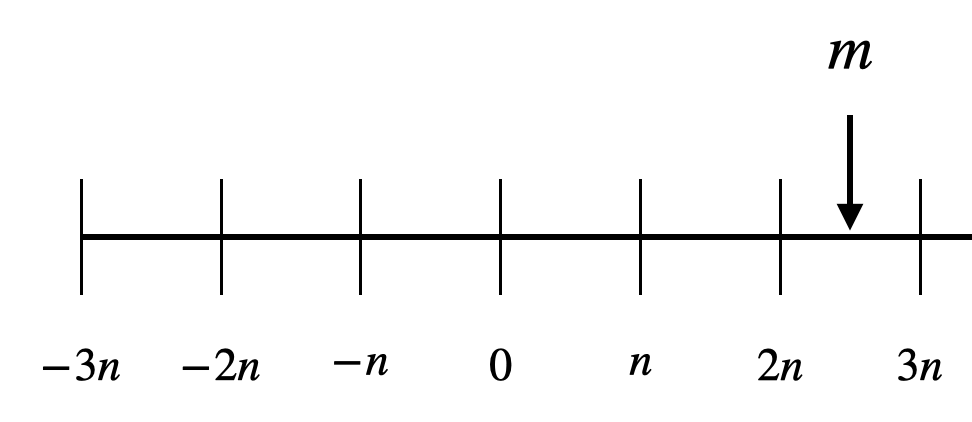
\includegraphics[width=0.7 \textwidth]{Int.png}
% \caption{\label{fig:Jesus}Jesus was uploaded via the file-tree menu.}
\end{figure}
\begin{flushleft}
    이 그림과 같은 경우, 연속적인 점들 사이의 거리는 $n$의 절댓값인 $\lvert n \rvert$ 입니다. 만일 $m$이 $n$의 배수라고 하면 $m = qn + r$이라고 쓸 수 있으며, $r = 0$ 입니다. 만약 $m$이 $n$의 배수가 아니면 $m = qn + r$이라고 쓰며, $0 < r< \lvert n \rvert$ 입니다. 
\end{flushleft}

\begin{tcolorbox}[colback = white, colframe = Definition, title = \textmd{정의: 정수 표현 방법}]
    두 정수 $m$, $n$에 대해서 모든 경우는 $m = qn + r$ 이며, $0 \leq r \leq \lvert n \rvert$ 으로 표현할 수 있다. (이때 $q$는 정수이다.)
\end{tcolorbox}

\bigskip
%%%%%%%%%%%%%%%%%%%%%%%%%%%%%%%%%%%%%%%%%%%%%%%%%% 정수의 성질 %%%%%%%%%%%%%%%%%%%%%%%%%%%%%%%%%%%%%%%%%%%%%%%%%%
\begin{flushleft}
    {\setmainhangulfont[Path=FONT/]{KOPUBWORLD_DOTUM_PRO_BOLD.OTF}\textcolor{subheader}{{\LARGE\textbf{정수의 성질}}}}
\end{flushleft}

\begin{flushleft}
    정수 표현에 있어서 중요한 배수 표현은 다음과 같습니다. 배수 표현을 통하여 정수의 성질도 도출해낼 수 있습니다. 
\end{flushleft}

\begin{tcolorbox}[colback = white, colframe = Definition, title = \textmd{정의: 배수 표현}]
    두 정수 $m$과 $n$에 대하여, $m$은 $n$의 배수이면 $n \ | \ m$ 이라 쓰며 $n$은 $m$을 나눈다라고 표현한다.
\end{tcolorbox}

\begin{tcolorbox}[colback = white, colframe = Theorem, title = \textmd{정리: 정수의 성질}]
    \begin{enumerate}
        \item 만일 $a \ | \ b$ 이고, $a \ | \ c$ 이면 $a \ | \ (b \pm c)$ 이다.
        \item 만일 $a \ | \ b$ 혹은, $a \ | \ c$ 이면 $a \ | \ bc$ 이다.
        \item 만일 $a \ | \ b$ 이고, $b \ | \ c$ 이면 $a \ | \ c$ 이다
    \end{enumerate}
\end{tcolorbox}

\newpage
%%%%%%%%%%%%%%%%%%%%%%%%% 소수와 합성수 %%%%%%%%%%%%%%%%%%%%%%%%%
\begin{flushleft}
    {\setmainhangulfont[Path=FONT/]{KOPUBWORLD_DOTUM_PRO_BOLD.OTF}\textcolor{subheader}{{\LARGE\textbf{소수와 합성수}}}}
\end{flushleft}

\begin{flushleft}
    소수는 현대 암호 시스템에서 필수적인 개념입니다. 특히 소수에 관한 내용 중 알아야 하는 것은 “소수 판별법”입니다. 그러나 현재까지는 어떤 수가 소수인지를 빠르게 계산하는 알고리즘을 찾지 못했습니다.
\end{flushleft}

\begin{tcolorbox}[colback = white, colframe = Definition, title = \textmd{정의: 소수}]
    약수(나누어떨어지는 수)로 $1$과 자기 자신만을 갖는 $1$보다 큰 정수 
    Ex: $2, \ 3, \ 5, \ 7 ...$
\end{tcolorbox}

\begin{tcolorbox}[colback = white, colframe = Definition, title = \textmd{정의: 합성수}]
    소수가 아닌 $1$보다 큰 정수 
    Ex: $4, \ 6, \ 8, \ 9 ...$
\end{tcolorbox}

\begin{flushleft}
    소수에 대한 내용은 추후에 더 깊고 자세하게 다루도록 하겠습니다.
\end{flushleft}
\newpage
% 2페이지
%%%%%%%%%%%%%%%%%%%%%%%%% 상단 제목 %%%%%%%%%%%%%%%%%%%%%%%%%
\begin{tikzpicture}[remember picture,overlay]
    \draw[fill = blue!40] (0.46,0) rectangle (25, 4); 
    \node[draw = blue!40] at (3, 1.7)  {\setmainhangulfont[Path=FONT/]{KOPUBWORLD_DOTUM_PRO_BOLD.OTF}{\textcolor{white}{{\huge 이산수학 개론}}}};  
    \node[draw = blue!40] at (5.3, 0.8)  {\setmainhangulfont[Path=FONT/]{KOPUBWORLD_DOTUM_PRO_MEDIUM.OTF}{\textcolor{white}{{\small 행과 열을 수학적으로 표기하는 기법인 행렬 대해서 알아봅시다.}}}};
    % (x축, y축)
\end{tikzpicture}

\begin{tikzpicture}[remember picture,overlay]
    \draw[fill = black!90] (-2.51, 3.4) rectangle (0.45, 0.55); 
    \node[] at (-1, 2.33) {\setmainfont[Path=FONT/]{KOPUBWORLD_BATANG_PRO_MEDIUM.OTF}{\textcolor{skyblue}{{\Huge {Alpha}}}}};
    \node[] at (-1, 1.45)  {\setmainfont[Path=FONT/]{KOPUBWORLD_BATANG_PRO_BOLD.OTF}{{\textcolor{skyblue}{{\Huge\textbf {1.2}}}}}};
\end{tikzpicture}

%%%%%%%%%%%%%%%%%%%%%%%%%%%%%%%%%%%%%%%%%%%%%%%%%% 행렬 %%%%%%%%%%%%%%%%%%%%%%%%%%%%%%%%%%%%%%%%%%%%%%%%%%

\begin{flushleft}
    {\setmainfont[Path=FONT/]{KOPUBWORLD_DOTUM_PRO_BOLD.OTF} {\textcolor{header}{{\huge\textbf{1.}}}}}
    {\setmainhangulfont[Path=FONT/]{KOPUBWORLD_DOTUM_PRO_BOLD.OTF} {\textcolor{header}{{\huge\textbf{행렬}}}}}
\end{flushleft}

\begin{flushleft}
    행렬은 행과 열로 나열하는 것을 말합니다. 기본적으로 연립방정식을 풀기 위하여 만들어진 개념이며, 수, 문자, 함수 등을 괄호 안에 배열한 것입니다. 행렬의 각 성분은 실수여야 하고, 이는 “스칼라(Scalar)”라고 합니다. 스칼라는 크기만 있고 방향을 가지지 않는 양을 말하며, 벡터와는 반대되는 개념입니다. 수학적으로 정의한 행렬은 다음과 같습니다. 
\end{flushleft}

\begin{tcolorbox}[colback = white, colframe = Definition, title = \textmd{정의: 행렬}]
    행렬 $A$는 실수들을 사각형의 배열로 표시한 것이다(단, $m$과 $n$은 양의 정수). 각각 $n$쌍으로 된 $m$개의 수평 성분 ($a_{i1} \ a_{i2} \ a_{i3} \cdots  a_{in} $) (단, $1 \leq i \leq m $)을 $A$의 행(row)이라고 하고, 각각 $m$쌍으로 된 $n$개의 수직 성분 ($a_{1j} \ a_{2j} \ a_{3j} \cdots  a_{mj} $)(단, $1 \leq j \leq n$)을 $A$의 열(column)이라고 한다.
    \[ A = \begin{pmatrix} a_{11} & a_{12} & a_{13} & \cdots & a_{1n} \\  
        a_{21} & a_{22} & a_{23} & \cdots  & a_{2n}  \\ && \vdots &&  \\
        a_{m1} & a_{m2} & a_{m3} & \cdots & a_{mn}\end{pmatrix}  \]
\end{tcolorbox}

\begin{flushleft}
행렬 $A$를 $A = (a_{ij})$로 표시하는데, 이때, 원소 $a_{ij}$는 $i$행의 $j$번째 열의 원소를 나타냅니다. $A$를 $m \times n$ 행렬이라고 하며, $m \ by \ n$ 행렬로 읽습니다.
\end{flushleft}

\bigskip
\begin{flushleft}
    {\setmainfont[Path=FONT/]{KOPUBWORLD_DOTUM_PRO_BOLD.OTF} {\textcolor{header}{{\huge\textbf{2.}}}}}
    {\setmainhangulfont[Path=FONT/]{KOPUBWORLD_DOTUM_PRO_BOLD.OTF} {\textcolor{header}{{\huge\textbf{행렬의 연산}}}}}
\end{flushleft}

\begin{flushleft}
    기초적인 행렬의 연산을 알아보기 전, "영행렬"과 "행렬의 같음 성질"에 대해서 알아야 합니다.
    먼저, 영행렬부터 알아보도록 하겠습니다.
\end{flushleft}

\bigskip
\begin{flushleft}
    {\setmainhangulfont[Path=FONT/]{KOPUBWORLD_DOTUM_PRO_BOLD.OTF}\textcolor{subheader}{{\LARGE\textbf{영행렬}}}}
\end{flushleft}

\begin{flushleft}
    만약 각 성분이 모두 0이라면, 이 행렬을 “영행렬”이라고 하고 0으로 표시합니다. 
\end{flushleft}

\begin{tcolorbox}[colback = white, colframe = Definition, title = \textmd{정의: 영행렬}]
    각 성분이 0인 행렬을 말한다. 영행렬은 $0$으로 표시한다.
    \[ \begin{pmatrix} 0 & 0 \\ 0 & 0 \end{pmatrix}, \ 
    \begin{pmatrix} 0 &0 & 0 \\ 0 & 0 & 0 \end{pmatrix}, \ 
    \begin{pmatrix} 0 & 0 & 0 \\ 0 & 0 & 0 \\ 0 & 0 & 0 \end{pmatrix} \]
\end{tcolorbox}

\bigskip
\begin{flushleft}
    {\setmainhangulfont[Path=FONT/]{KOPUBWORLD_DOTUM_PRO_BOLD.OTF}\textcolor{subheader}{{\LARGE\textbf{두 행렬의 같음}}}}
\end{flushleft}

\begin{flushleft}
    두 행렬이 있을 때, 그 두 행렬이 같을 조건은 다음과 같습니다.
\end{flushleft}

\begin{tcolorbox}[colback = white, colframe = Definition, title = \textmd{정의: 두 행렬의 같음}]
    두 행렬이 $m \times n$ 행렬이고 대응하는 원소가 모두 같으면 $A = (a_{ij})$와 $B = (b_{ij})$는 같다라고 하며, $A = B$ 라고 표현한다.
\end{tcolorbox}

\newpage

\begin{flushleft}
    지금부터는 본격적인 행렬의 연산 방식에 대해 알아보도록 하겠습니다. 행렬의 기초적인 연산으로는 행렬의 덧셈, 행렬의 실수곱, 행렬곱 등이 있습니다.
\end{flushleft}

\bigskip
\begin{flushleft}
    {\setmainhangulfont[Path=FONT/]{KOPUBWORLD_DOTUM_PRO_BOLD.OTF}\textcolor{subheader}{{\LARGE\textbf{행렬의 합}}}}
\end{flushleft}

\begin{flushleft}
    행렬의 합은 다음과 같이 정의합니다.
\end{flushleft}

\begin{tcolorbox}[colback = white, colframe = Definition, title = \textmd{정의: 행렬의 합}]
    행렬 $A$와 $B$가 같은 크기와 행과 열을 가지면, 행렬 $A$와 $B$의 행렬의 합은 $A + B$로 표시하고 $A + B = (a_{ij}) + (b_{ij}) = (a_{ij}+b_{ij})$이다. 즉, 대응하는 성분끼리 합을 구하면 그 값이 $A + B$의 각 성분이 되는 것이다.
\end{tcolorbox}

\begin{flushleft}
    행렬의 합을 통하여 알 수 있는 행렬의 덧셈 성질은 다음과 같다.
\end{flushleft}

\begin{tcolorbox}[colback = white, colframe = Theorem, title = \textmd{정리: 행렬의 덧셈 성질}]
    \begin{enumerate}
        \item $A + B = B + A$    (덧셈의 교환법칙)
        \item $(A + B) + C = A + (B + C)$    (덧셈의 결합법칙)
        \item $A + 0 = 0 + A = A$    (덧셈의 항등법칙)
    \end{enumerate}
\end{tcolorbox}

\newpage
\begin{flushleft}
    {\setmainhangulfont[Path=FONT/]{KOPUBWORLD_DOTUM_PRO_BOLD.OTF}\textcolor{subheader}{{\LARGE\textbf{스칼라 곱과 행렬의 곱}}}}
\end{flushleft}

\begin{flushleft}
    스칼라 곱은 행렬에 실수배를 하는 것입니다. 스칼라 곱은 다음과 같이 정의됩니다.
\end{flushleft}

\begin{tcolorbox}[colback = white, colframe = Definition, title = \textmd{정의: 스칼라 곱}]
    $A$가 $m \times n$ 행렬이고 $c$가 실수이면 다음이 성립한다.
    $$ c \cdot A = c \cdot (a_{ij}) = (c \times a_{ij}) $$  
\end{tcolorbox}

\begin{flushleft}
    두 행렬을 곱하는 행렬의 곱은 다음과 같이 정의됩니다.
\end{flushleft}

\begin{tcolorbox}[colback = white, colframe = Definition, title = \textmd{정의: 행렬의 곱}]
    $A = (a_{ij})$는 $m \times p $ 행렬이고 $B = (b_{ij})$는 $p \times n$ 행렬일 때, 행렬의 곱 $AB$는 $m \times n $ 행렬이고 $C = (c_{ij})$가 된다. 이때, 
    \[ C_{ij} = a_{i1}b_{1j} + a_{i2}b_{2j} \cdots + a_{ip}b_{pj} \quad (\text{단, } 1 \leq i \leq m, \ 1 \leq j \leq n) \]
    이다. 즉, 행렬의 곱 $AB$는 다음과 같이 구할 수 있다. \\

    $ AB = \begin{pmatrix} a_{11} & a_{12} & \cdots & a_{1p} \\  
    a_{21} & a_{22} & \cdots  & a_{2p}  \\ && \vdots  \\ 
    a_{i1} & a_{i2} & \cdots & a_{ip}
    \\  && \vdots   \\ 
    a_{m1} & a_{m2} & \cdots & a_{mp}\end{pmatrix} $
    $ \begin{pmatrix} b_{11} & b_{12} &  \cdots b_{1j} & \cdots & b_{1n} \\  
    b_{21} & b_{22} & \cdots b_{1j} & \cdots & b_{2n}  \\ && \vdots &&  \\ && \vdots &&  \\ && \vdots &&  \\
    b_{p1} & b_{p2} & \cdots b_{1j} & \cdots & b_{pn}\end{pmatrix} $
    =
    $ \begin{pmatrix} c_{11} & c_{12} & c_{13} & \cdots & c_{1n} \\  
    c_{21} & c_{22} & c_{23} & \cdots  & c_{2n}  \\ && \vdots &&  \\ 
    & \cdots & c_{ij} & \cdots 
    \\ && \vdots &&  \\ 
    c_{m1} & c_{m2} & c_{m3} & \cdots & c_{mn}\end{pmatrix} $
\end{tcolorbox}

\begin{flushleft}
    행렬의 곱을 통하여 알 수 있는 행렬의 곱셈 성질은 다음과 같습니다.
\end{flushleft}

\begin{tcolorbox}[colback = white, colframe = Theorem, title = \textmd{정리: 행렬의 곱셈 성질}]
    \begin{enumerate}
        \item $A \cdot (B \cdot C) = (A \cdot B) \cdot C$    (곱셈의 결함법칙)
        \item $A \cdot (B + C) = A \cdot B +A \cdot C$    (곱셈의 분배법칙)
        \item $(A + B) \cdot C = A \cdot C + B \cdot C$    (곱셈의 분배법칙)
    \end{enumerate}
\end{tcolorbox}

\newpage
\begin{flushleft}
    {\setmainfont[Path=FONT/]{KOPUBWORLD_DOTUM_PRO_BOLD.OTF} {\textcolor{header}{{\huge\textbf{3.}}}}}
    {\setmainhangulfont[Path=FONT/]{KOPUBWORLD_DOTUM_PRO_BOLD.OTF} {\textcolor{header}{{\huge\textbf{특수 행렬}}}}}
\end{flushleft}

\begin{flushleft}
    지금부터 여러 종류의 행렬들에 대해서 하나하나 알아보도록 하겠습니다. 양이 많기에 모든 행렬을 일일이 외우기보다, "이런 행렬들도 있구나" 하고 눈에 익히는 정도로만 공부하면 됩니다.
\end{flushleft}

\bigskip
\begin{flushleft}
    {\setmainhangulfont[Path=FONT/]{KOPUBWORLD_DOTUM_PRO_BOLD.OTF}\textcolor{subheader}{{\LARGE\textbf{정방 행렬}}}}
\end{flushleft}

\begin{tcolorbox}[colback = white, colframe = Definition, title = \textmd{정의: 정방 행렬}]
    행과 열의 수가 $n$으로 같은 행렬을 $n$차 정방 행렬이라고 한다. 이때, 행 또는 열의 개수를 “정방 행렬의 차수”라고 하며, $n$차 정방 행렬에서 대각선상에 위치한 원소, $a_{ii}(i = 1, \ 2, \ 3, \cdots, \ n)$를 “주대각 원소”라고 한다. 
\end{tcolorbox}

\bigskip
\begin{flushleft}
    {\setmainhangulfont[Path=FONT/]{KOPUBWORLD_DOTUM_PRO_BOLD.OTF}\textcolor{subheader}{{\LARGE\textbf{단위 행렬(항등 행렬)}}}}
\end{flushleft}

\begin{tcolorbox}[colback = white, colframe = Definition, title = \textmd{정의: 단위 행렬(항등 행렬)}]
    주대각 원소들은 모두 $1$이고, 주대각 원소를 제외한 나머지 원소들은 모두 $0$인 정방 행렬을 단위 행렬 또는 항등 행렬이라고 한다.
    \[ \begin{pmatrix} 1 & 0 \\ 0 & 1 \end{pmatrix}, \ 
    \begin{pmatrix} 1 & 0 & 0 \\ 0 & 1 & 0 \\ 0 & 0 & 1 \end{pmatrix} \]
\end{tcolorbox}

\bigskip
\begin{flushleft}
    {\setmainhangulfont[Path=FONT/]{KOPUBWORLD_DOTUM_PRO_BOLD.OTF}\textcolor{subheader}{{\LARGE\textbf{대각 행렬}}}}
\end{flushleft}

\begin{tcolorbox}[colback = white, colframe = Definition, title = \textmd{정의: 대각 행렬}]
    주대각 원소를 제외한 나머지 원소가 모두 $0$인 행렬을 대각 행렬이라고 한다. 
    \[ \begin{pmatrix} 2 & 0 \\ 0 & 3 \end{pmatrix}, \ 
    \begin{pmatrix} 2 & 0 & 0 \\ 0 & 3 & 0 \\ 0 & 0 & 4 \end{pmatrix} \]
\end{tcolorbox}


\bigskip
\begin{flushleft}
    {\setmainhangulfont[Path=FONT/]{KOPUBWORLD_DOTUM_PRO_BOLD.OTF}\textcolor{subheader}{{\LARGE\textbf{스칼라 행렬}}}}
\end{flushleft}

\begin{tcolorbox}[colback = white, colframe = Definition, title = \textmd{정의: 스칼라 행렬}]
    주대각 원소들이 모두 같은 값을 갖는 대각 행렬을 스칼라 행렬이라고 한다.
    \[ \begin{pmatrix} 3 & 0 \\ 0 & 3 \end{pmatrix}, \ 
    \begin{pmatrix} 5 & 0 & 0 \\ 0 & 5 & 0 \\ 0 & 0 & 5 \end{pmatrix} \]
\end{tcolorbox}

\newpage
\begin{flushleft}
    {\setmainhangulfont[Path=FONT/]{KOPUBWORLD_DOTUM_PRO_BOLD.OTF}\textcolor{subheader}{{\LARGE\textbf{전치 행렬}}}}
\end{flushleft}

\begin{tcolorbox}[colback = white, colframe = Definition, title = \textmd{정의: 전치 행렬}]
    행렬 $A$가 임의의 $m \times n$ 행렬일 때, $A$의 행과 열을 바꾼 $n \times m$ 행렬을 전치행렬이라고 한다. $A$의 전치행렬은 $A^T$라고 표현한다.
\end{tcolorbox}

\bigskip
\begin{flushleft}
    {\setmainhangulfont[Path=FONT/]{KOPUBWORLD_DOTUM_PRO_BOLD.OTF}\textcolor{subheader}{{\LARGE\textbf{대칭 행렬}}}}
\end{flushleft}

\begin{tcolorbox}[colback = white, colframe = Definition, title = \textmd{정의: 대칭 행렬}]
    어떤 정방 행렬이 자신과 자신의 전치 행렬이 같으면 그 행렬을 대칭 행렬이라고 한다. 행렬 $A$가 대칭 행렬이면 $A = A^T$를 만족한다.
\end{tcolorbox}

\bigskip
\begin{flushleft}
    {\setmainhangulfont[Path=FONT/]{KOPUBWORLD_DOTUM_PRO_BOLD.OTF}\textcolor{subheader}{{\LARGE\textbf{띠 행렬}}}}
\end{flushleft}

\begin{tcolorbox}[colback = white, colframe = Definition, title = \textmd{정의: 띠 행렬}]
    주대각 원소와 평행한 몇 줄의 원소들만 값을 갖고, 그 이외의 모든 원소들은 $0$인 행렬을 띠 행렬이라고 한다.
    \[ \begin{pmatrix} 5 & 4 & 0 \\ 6 & 7 & 2 \\ 0 & 9 & 3 \end{pmatrix}, 
    \begin{pmatrix} 5 & 4 & 0 & 0 \\ 0 & 7 & 2 & 0 \\ 0 & 0 & 3 & 8 \\ 0 & 0 & 0 & 9\end{pmatrix} \]
\end{tcolorbox}

\bigskip
\begin{flushleft}
    {\setmainhangulfont[Path=FONT/]{KOPUBWORLD_DOTUM_PRO_BOLD.OTF}\textcolor{subheader}{{\LARGE\textbf{삼각 행렬}}}}
\end{flushleft}

\begin{flushleft}
    상삼각 행렬이거나 하삼각 행렬을 간단하게 삼각 행렬이라고 합니다.
\end{flushleft}

\begin{tcolorbox}[colback = white, colframe = Definition, title = \textmd{정의: 상삼각 행렬}]
    주대각 원소의 아래쪽에 있는 모든 원소들이 $0$인 정방 행렬을 상삼각 행렬이라고 한다.
    \[ \begin{pmatrix} 3 & 5 \\ 0 & 4 \end{pmatrix}, \ 
    \begin{pmatrix} 5 & 6 & 7 \\ 0 & 8 & 9 \\ 0 & 0 & 3 \end{pmatrix} \]
\end{tcolorbox}
\begin{tcolorbox}[colback = white, colframe = Definition, title = \textmd{정의: 하삼각 행렬}]
    주대각 원소의 위쪽에 있는 모든 원소들이 $0$인 정방 행렬을 하삼각 행렬이라고 한다.
    \[ \begin{pmatrix} 3 & 0 \\ 5 & 4 \end{pmatrix}, \ 
    \begin{pmatrix} 5 & 0 & 0 \\ 6 & 7 & 0 \\ 8 & 9 & 3 \end{pmatrix} \]
\end{tcolorbox}

\newpage
\begin{flushleft}
    {\setmainhangulfont[Path=FONT/]{KOPUBWORLD_DOTUM_PRO_BOLD.OTF}\textcolor{subheader}{{\LARGE\textbf{역행렬}}}}
\end{flushleft}
\begin{tcolorbox}[colback = white, colframe = Definition, title = \textmd{정의: 역행렬}]
    임의의 정방 행렬 $A$에 대하여, $AB = BA = I$를 만족하는 정방 행렬 $B$가 존재할 때 $A$는 "가역"(역행렬이 존재함)이라고 하고, $B$는 $A$의 역행렬이라고 하며 $A^{-1}$로 표시한다.
\end{tcolorbox}
\begin{tcolorbox}[colback = white, colframe = Theorem, title = \textmd{정리: 2차 정방 행렬의 역행렬 }]
    2차 정방 행렬 $A = \begin{pmatrix} a & b\\ c & d  \end{pmatrix}$는 $\text{det}(A) = ad - bc \ne 0$이므로 가역이고, $A$의 역행렬은 다음과 같이 구한다.
    \[ A^{-1} = \frac{1}{ad - bc} \begin{pmatrix} d & -b \\ -c & a \end{pmatrix} \]
\end{tcolorbox}
\begin{flushleft}
    역행렬을 구하는 방법은 아주 다양합니다. 일반적으로 연립방정식을 이용하여 푸는데, 연립방정식을 푸는 방법은 가우스 소거법, 가우스-조단 방법 같이 직접적인 해를 구하는 방법과 야코비 방법, 가우스-자이델 방법 같이 반복적으로 해를 구하는 방법이 있습니다. 
    이에 대한 자세한 공부는 다음에 다루고 지금은 넘어가도록 하겠습니다.
\end{flushleft}

\bigskip
\begin{flushleft}
    {\setmainhangulfont[Path=FONT/]{KOPUBWORLD_DOTUM_PRO_BOLD.OTF}\textcolor{subheader}{{\LARGE\textbf{정칙 행렬}}}}
\end{flushleft}

\begin{tcolorbox}[colback = white, colframe = Definition, title = \textmd{정의: 정칙 행렬}]
    임의의 정방 행렬 $A$가 있을 때, $A$의 역행렬이 존재하는 행렬을 정칙 행렬이라고 한다. $\text{det} (A) \neq 0$이 되는 행렬을 말한다.    
    \[ \begin{pmatrix} 1 & 3 \\ 2 & 4 \end{pmatrix} \]
\end{tcolorbox}

\bigskip
\begin{flushleft}
    {\setmainhangulfont[Path=FONT/]{KOPUBWORLD_DOTUM_PRO_BOLD.OTF}\textcolor{subheader}{{\LARGE\textbf{직교 행렬}}}}
\end{flushleft}

\begin{tcolorbox}[colback = white, colframe = Definition, title = \textmd{정의: 직교 행렬}]
    임의의 행렬 $A$에 대하여, $A^{-1} = A^{T}$가 되는 행렬을 직교 행렬이라고 한다.
\end{tcolorbox}

\bigskip
\begin{flushleft}
    {\setmainhangulfont[Path=FONT/]{KOPUBWORLD_DOTUM_PRO_BOLD.OTF}\textcolor{subheader}{{\LARGE\textbf{특이 행렬}}}}
\end{flushleft}

\begin{tcolorbox}[colback = white, colframe = Definition, title = \textmd{정의: 특이 행렬}]
    임의의 정방 행렬 $A$가 있을 때, $A$의 역행렬이 존재하지 않는 행렬을 특이 행렬이라고 한다. $\text{det} (A) = 0$이 되는 행렬을 말한다.
    \[ \begin{pmatrix} 1 & 4 & 0 \\ 2 & 5 & 0 \\ 3 & 6 & 0 \end{pmatrix} \]
\end{tcolorbox}

\newpage
\begin{flushleft}
    {\setmainhangulfont[Path=FONT/]{KOPUBWORLD_DOTUM_PRO_BOLD.OTF}\textcolor{subheader}{{\LARGE\textbf{부울 행렬}}}}
\end{flushleft}

\begin{tcolorbox}[colback = white, colframe = Definition, title = \textmd{정의: 부울 행렬}]
    행렬의 원소들이 $0$이거나 $1$인 $m \times n$ 행렬을 부울 행렬이라고 한다.
\end{tcolorbox}

\begin{flushleft}
    부울 행렬의 연산과 부울 연산은 다른데, 부울 행렬에서 사용하는 연산자는 “접합”, “교합”, “부울곱”입니다.
\end{flushleft}

\begin{tcolorbox}[colback = white, colframe = Definition, title = \textmd{정의: 접합}]
    $A = (a_{ij}), \ B = (b_{ij})$인 $m \times n$ 부울 행렬이 존재할 때,
    $A \vee B = C = (C_{ij})$를 $A$와 $B$의 접합이라고 하며, 다음과 같이 정의한다.
    \[ (c_{ij}) =  
    \begin{cases}
        1, \quad a_{ij}= 1 \text{ 혹은 } b_{ij} = 1 \ 인 \ 경우  \\
        0, \quad a_{ij} \ 와 \ b_{ij} \ 가 \ 모두 \ 0 \ 인 \ 경우 \\
    \end{cases} \]
\end{tcolorbox}

\begin{tcolorbox}[colback = white, colframe = Definition, title = \textmd{정의: 교합}]
    $A = (a_{ij}), \ B = (b_{ij})$인 $m \times n$ 부울 행렬이 존재할 때,
    $A \wedge B = D = (d_{ij})$를 $A$와 $B$의 교합이라고 하며, 다음과 같이 정의한다.
    \[ (d_{ij}) =  
    \begin{cases}
        1, \quad a_{ij} \ 와 \ b_{ij} \ 가 \ 모두 \ 1 \ 인 \ 경우 \\
        0, \quad a_{ij}= 0 \text{ 혹은 } b_{ij} = 0 \ 인 \ 경우
    \end{cases} \]
\end{tcolorbox}

\begin{tcolorbox}[colback = white, colframe = Definition, title = \textmd{정의: 부울곱}]
    $E \odot F = G = (g_{ij})$를 $E$와 $F$의 부울곱이라고 한다. 행렬 $E = (e_{ik})$가 $m \times p$ 부울 행렬이고 
    $F = (f_{ij})$가 $p \times n$ 부울 행렬이면 $E$와 $F$의 부울곱은 $m\times n$ 부울 행렬이 되고 다음과 같이 정의한다.
    \[ (g_{ij}) =  
    \begin{cases}
        1, \quad 어떤 \ k(1 \leq k \leq p) \ 에 \ 대해  \ a_{ij}= 1,\ b_{ij} = 1 \ 인 \ 경우  \\
        0, \quad 그 \ 외에
    \end{cases} \]
\end{tcolorbox}

\begin{tcolorbox}[colback = white, colframe = Theorem, title = \textmd{정리: 부울 행렬의 성질}]
    $A, \ B, \ C$가 부울 행렬일 때, 다음 성질이 성립한다.
    \begin{itemize}
        \item $A \vee B = B \vee A \\ A \wedge B = B \wedge A  $ (교환법칙)
        \item $(A \vee B ) \vee C = A \vee (B\vee C) \\ (A \wedge B ) \wedge C = A \wedge (B\wedge C)$ (결합법칙)
        \item $A \wedge (B\vee C) = (A \wedge B) \vee (A \wedge C) \\ A \vee (B\wedge C) = (A \vee B) \wedge (A \vee C) $ (분배법칙)
        \item $A \odot (B \odot C)= (A \odot B) \odot C$ (결합법칙)
    \end{itemize}
\end{tcolorbox}

\newpage
\begin{flushleft}
    {\setmainfont[Path=FONT/]{KOPUBWORLD_DOTUM_PRO_BOLD.OTF} {\textcolor{header}{{\huge\textbf{4.}}}}}
    {\setmainhangulfont[Path=FONT/]{KOPUBWORLD_DOTUM_PRO_BOLD.OTF} {\textcolor{header}{{\huge\textbf{행렬식}}}}}
\end{flushleft}

\begin{flushleft}
    행렬식은 기본적으로 행렬의 역행렬을 구하기 위하여 주로 사용됩니다.
\end{flushleft}

\begin{tcolorbox}[colback = white, colframe = Definition, title = \textmd{정의: 행렬식}]
    행렬식은 모든 정방 행렬 $A$에 대하여 고유한 수치 값을 대응시키는 것을 말하며, $A$의 행렬식을 $\lvert A \rvert$ 또는 $\text{det}(A)$로 표시합니다.
    $2\times 2$인 행렬의 행렬식은 다음과 같이 정의합니다.
    \[ \text{det}\begin{pmatrix} a_{11} & a_{12} \\ a_{21} & a_{22}
    \end{pmatrix} = a_{11}a_{22} - a_{12}a_{21} \]
\end{tcolorbox}

\begin{flushleft}
    일반적인 행렬에 대한 행렬식은 사루스 법칙으로 구할 수 있습니다.
\end{flushleft}

\begin{tcolorbox}[colback = white, colframe = Theorem, title = \textmd{정리: 사루스 법칙}]
    $3 \times 3$ 행렬에서 사용되는 행렬을 구하는 공식이다. (사루스 법칙은 계산을 위한 공식으로 수학 공부 할 때는 그다지 추천하지 않는 공식입니다.)
    \[ \begin{vmatrix} a_{11} & a_{12} & a_{13} \\ a_{21} & a_{22} & a_{23} \\ a_{31} & a_{32} & a_{33}
    \end{vmatrix} = a_{11}a_{22}a_{33} + a_{12}a_{23}a_{31} + a_{13}a_{21}a_{32} - a_{13}a_{22}a_{31} - a_{12}a_{21}a_{33} - a_{11}a_{23}a_{32} \]
\end{tcolorbox}

\bigskip
\begin{flushleft}
    {\setmainhangulfont[Path=FONT/]{KOPUBWORLD_DOTUM_PRO_BOLD.OTF}\textcolor{subheader}{{\LARGE\textbf{행렬식에 관한 성질}}}}
\end{flushleft}


\begin{flushleft}
    다음은 행렬식에 관한 몇 가지 성질들입니다.
\end{flushleft}

\begin{tcolorbox}[colback = white, colframe = Theorem, title = \textmd{정리: 행렬식에 관한 몇 가지 성질}]
    $A, \ B, \ C$가 부울 행렬일 때, 다음 성질이 성립한다.
    \begin{itemize}
        \item 행렬 $A$의 각 원소의 행과 열이 바뀌어도 $\text{det}(A)$는 변하지 않는다.
        \item 행렬식에서 두 개의 행이나 열을 서로 바꾸면 부호만 변한다.
        \item 행렬 $A$가 서로 비례하는 두 개의 행 또는 두 개의 열을 갖는 정방 행렬이면 $\text{det}(A) = 0$이다.
        \item 행렬식에서 특정 어느 행이나 열의 각 성분이 두 수의 합일 때, 두 개의 행렬식의 합으로 나눌 수 있다.
    \end{itemize}
\end{tcolorbox}

\bigskip
\begin{flushleft}
    {\setmainhangulfont[Path=FONT/]{KOPUBWORLD_DOTUM_PRO_BOLD.OTF}\textcolor{subheader}{{\LARGE\textbf{소행렬식과 여인수}}}}
\end{flushleft}

\begin{flushleft}
    간단한 행렬의 행렬식은 사루스 법칙으로 계산할 수 있지만, 행렬의 크기가 커지면 계산하기 쉽지 않습니다. 
    이러한 문제점을 해결하기 위해 행렬식을 “소행렬식”과 “여인수”를 사용하여 계산하는 방법이 고안되었습니다.
\end{flushleft}

\begin{tcolorbox}[colback = white, colframe = Definition, title = \textmd{정의: 소행렬식}]
    행렬식에서 한 원소의 소행렬식은 그 원소가 있는 행과 열을 제외시킨 행렬식이다. 
행렬식이 $\begin{vmatrix} a_{11} & a_{12} & a_{13} \\ a_{21} & a_{22} & a_{23} \\ a_{31} & a_{32} & a_{33}
\end{vmatrix} $이렇게 주어진다면 $a_{11}$의 소행렬식은 $\begin{vmatrix}  a_{22} & a_{23} \\  a_{32} & a_{33}
\end{vmatrix} $이다.
\end{tcolorbox}

\begin{tcolorbox}[colback = white, colframe = Definition, title = \textmd{정의: 여인수}]
    하나의 정방 행렬에서 한 원소의 여인수는 그 원소의 소행렬식에 부호를 붙인 값을 말한다. 
    즉, 행렬 $A$의 $i$번째 행과 $j$번째 열을 제거해 만든 소행렬 $A_{ij}$의 행렬식 $\begin{vmatrix} A_{ij} \end{vmatrix}$에 부호 $(-1)^{i+j}$을 붙인 값을 $A$의 $i, \ j$번째 여인수라고 한다. 부호는 다음과 같이 붙인다.
    \[ \begin{vmatrix} + & - & + & \cdots \\ - &+ & - &  \cdots  \\ + & - & + & \cdots \\ \vdots  & \vdots  & \vdots 
    \end{vmatrix}  \]
\end{tcolorbox}

\begin{tcolorbox}[colback = white, colframe = Theorem, title = \textmd{정리: 여인수 전개(라플라스 전개)}]
    $M_{ij}$를 원소 $a_{ij}$의 소행렬식이라고 하면  $a_{ij}$의 여인수 $C_{ij} = (-1)^{i+ j}M_{ij}$이다. 
    또한, 행렬식 $\begin{vmatrix} A \end{vmatrix}$를 $n$행에 대해서 전개하면 다음과 같다.
    \[ \text{det}(A) = a_{n1}\begin{vmatrix} A_{n1} \end{vmatrix} + a_{n2}\begin{vmatrix} A_{n2} \end{vmatrix} + \cdots + a_{nn}\begin{vmatrix} A_{nn} \end{vmatrix} \]
    같은 방법으로 행렬식 $\begin{vmatrix} A \end{vmatrix}$를 $n$열에 대해서 전개하면 다음과 같다.
    \[ \text{det}(A) = a_{1n}\begin{vmatrix} A_{1n} \end{vmatrix} + a_{2n}\begin{vmatrix} A_{2n} \end{vmatrix} + \cdots + a_{nn}\begin{vmatrix} A_{nn} \end{vmatrix} \]
\end{tcolorbox}
\newpage
% 3페이지
%%%%%%%%%%%%%%%%%%%%%%%%%%%%%%%%%%%%%%%%%%%%%%%%%% 상단 제목 %%%%%%%%%%%%%%%%%%%%%%%%%%%%%%%%%%%%%%%%%%%%%%%%%%
\begin{tikzpicture}[remember picture,overlay]
    \draw[fill = blue!40] (0.46,0) rectangle (25, 4); 
    \node[draw = blue!40] at (3.4, 1.7)  {\setmainhangulfont[Path=FONT/]{KOPUBWORLD_DOTUM_PRO_BOLD.OTF}{\textcolor{white}{{\huge 명제와 논리 연산}}}};  
    \node[draw = blue!40] at (5.3, 0.8)  {\setmainhangulfont[Path=FONT/]{KOPUBWORLD_DOTUM_PRO_MEDIUM.OTF}{\textcolor{white}{{\small 다양한 명제의 종류와 여러 논리 연산 방법에 대해 알아봅시다.}}}};
    % (x축, y축)
\end{tikzpicture}

\begin{tikzpicture}[remember picture,overlay]
    \draw[fill = black!90] (-2.51, 3.4) rectangle (0.45, 0.55); 
    \node[] at (-1, 2.33) {\setmainfont[Path=FONT/]{KOPUBWORLD_BATANG_PRO_MEDIUM.OTF}{\textcolor{skyblue}{{\Huge {Alpha}}}}};
    \node[] at (-1, 1.45)  {\setmainfont[Path=FONT/]{KOPUBWORLD_BATANG_PRO_BOLD.OTF}{{\textcolor{skyblue}{{\Huge\textbf {2.1}}}}}};
\end{tikzpicture}

\newpage

\end{document}

